\documentclass[a4paper]{article}
\usepackage{amsmath,amssymb,enumerate, graphicx,amsfonts, makeidx, hyperref}
\begin{document}
\begin{center}

{\bf{\huge Math 461 }}\\
\vspace{ 0.5 cm }
{\bf{\huge a.k.a. }}\\
\vspace{ 0.5 cm }
{\bf{\huge Probability }}\\
\vspace{ 5 cm }
{\bf{\large Spring 2012, University of Illinos}}\\
{\bf{\large as taught by Peter Loeb}}\\
\vspace{ 1 cm }                         
{\large notes by Michele R. Esposito}\\
\vspace{ 5cm }
Please, let report any error or type-o at\\
\underline{\href{mailto:micheleresposito@gmail.com}{ micheleresposito@gmail.com }}
\end{center}
\newpage
\tableofcontents
\newpage

% =========================================================
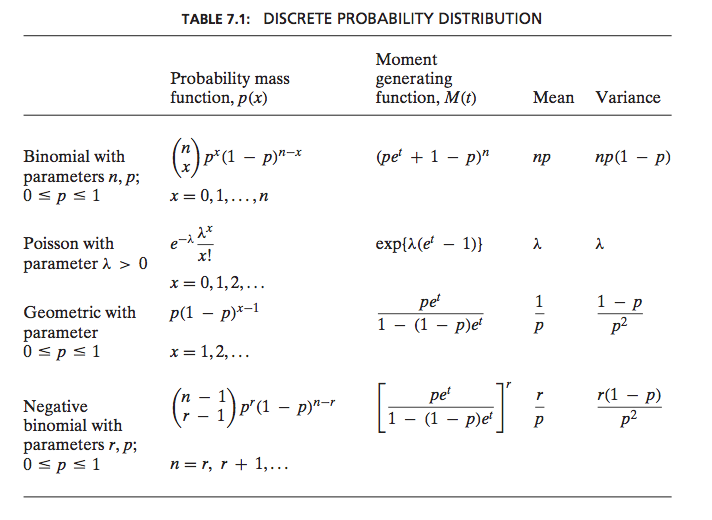
\includegraphics[scale=.50]{table1.png} \\
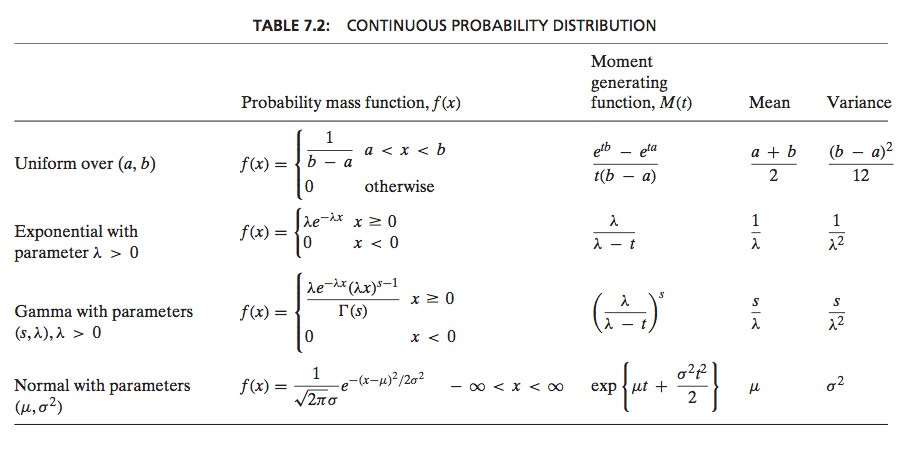
\includegraphics[scale=.50]{table2.png}

\section{Chapter 1: Combinatorial Analysis} % (fold)
\label{sec:Chapter 1: Combinatorial Analysis}
\subsection{The basic principle of counting} % (fold)
\label{sub:The Basic principle of counting}
Suppose that two experiments are to be performed. Then if experiment 1 can result in any one of $m$ possible outcomes and if,
for each outcome of experiment 1, there are $n$ possible outcomes of experiment 2, then together there are $mn$ possible
outcomes of the two experiments.
% subsection The Basic principle of counting (end)
\subsection{Permutations} % (fold)
\label{sub:Permutations}
Suppose that we have $n$ objects. We are then going to have $n!$ different permutations of the $n$ objects.
% subsection Permutations (end)
\subsection{Combinations} % (fold)
\label{sub:Combinations}
In general, as $n(n-1)\dots (n-r+1)$ represents the number of different ways that a group of $r$ items could be selected from $n$
items when the order of selection is relevant, and as each group of $r$ items will be counted $r!$ times in this count, it follows
that the number of different groups of $r$ items that could be formed from a set of $n$ items is: \\
\begin{align}
    \frac{n(n-1)\dots (n-r+1)}{r!}= \frac{n!}{(n-r)!r!}= { n \choose r } 
\end{align}
\subsubsection{The binomial theorem} % (fold)
\label{sub:The binomial theorem}

\begin{center}
  $(x+y)^n = \sum^n_{k=0} { n \choose k} x^k y^{n-k} $
\end{center}
% subsubsection The binomial theorem (end)
% subsection Combinations (end)
\subsection{Multinomial Coefficients} % (fold)
\label{sub:Multinomial Coefficients}
If $n_1+n_2+ \dots + n_r = n$, we define ${ n \choose n_1,n_2,\dots, n_r}$ by
\begin{align}
  { n \choose n_1,n_2,\dots, n_r} = \frac{n!}{n_1!n_2! \dots n_r!}
\end{align}
Thus, ${ n \choose n_1,n_2,\dots, n_r}$ represents the number of possible divisions of $n$ distinct objects into $r$ distinct groups of respective sizes $n_1,n_2, \dots n_r$.
% subsection Multinomial Coefficients (end)
\subsection{The multinomial theorem} % (fold)
\label{sub:The multinomial theorem}
\begin{align}
  (x_1+x_2+\dots + x_r)^n = \sum_{(n_1,\dots,n_r):n_1+\dots+n_r=n} { n \choose n_1,n_2,\dots, n_r}x_1^{n_1}x_2^{n_2}\dots x_r^{n_r}
\end{align}
That is, the sum is over all nonnegative integer-valued vectors $(n_1,n_2,\dots, n_r)$ such that $n_1+n_2+\dots+n_r = n$.
% subsection The multinomial theorem (end)
\subsection{Number of integer solutions of equations} % (fold)
\label{sub:Number of integer solutions of equations}
There are ${ n-1 \choose r-1 }$ distinct positive integer-valued vectors $(x_1,x_2,\dots, x_r)$ satisfying the equation
\begin{align}
  x_1,x_2,\dots, x_r = n \text{    } x_i > 0, i=1,\dots, r
\end{align}

There are ${ n+r-1 \choose r-1 }$ distinct nonnegative integer-valued vectors $(x_1,x_2,\dots, x_r)$ satisfying the equation
\begin{align}
  x_1,x_2,\dots, x_r = n 
\end{align}
% subsection Number of integer solutions of equations (end)
% section Chapter 1: Combinatorial Analysis (end)
% =========================================================

% =========================================================
% =========================================================
% =========================================================
\section{Axioms of Probability} % (fold)
\label{sec:Axioms of Probablity}
\subsection{Sample space and events} % (fold)
\label{sub:Sample space and events}
{\bf Sample space:} Set of all possible outcomes of an experiment. \\
{\bf Set laws:}
\begin{center}
  Cumulative Laws: $E \cup F = F \cup E   \;\;\;\;$          $EF = FE$ \\
  Associative Laws: $(E \cup F)\cup G= E \cup F(\cup G) \;\;\;\;$        $(EF)G=E(FG)$ \\
  Distributive laws:$(E \cup F) G = EG \cup FG\;\;\;\;$     $EF\cup G = (E\cup G)(F \cup G)$ \\
  De Morgan's Laws: $(\bigcup_{i=1}^n E_i )^c = \bigcap_{i=1}^n E_i^c \;\;\;\;$     $(\bigcap_{i=1}^n E_i )^c = \bigcup_{i=1}^n E_i^c$
\end{center}
% subsection Sample space and events (end)
\subsection{Axioms of probability} % (fold)
\label{sub:Axioms of probability}
The most intuitive definition of a probability is:
\begin{align}
  P(E)= \lim_{n \rightarrow \infty} \frac{n(E)}{n} 
\end{align}
Although, this is very unpractical to use. Thus, we have three axioms of probability: \\
{\bf Axiom 1:}
\begin{align}
  0 \leq P(E) \leq 1
\end{align}
{\bf Axiom 2:}
\begin{align}
  P(S)=1
\end{align}
{\bf Axiom 3:}
For any sequence of mutually exclusive events $E_1,E_2,\dots$ (that is, events for which $E_iE_j=\varnothing$ when $i \neq j$)
\begin{align}
  P(\bigcup_{i=1}^{\infty} E_i) = \sum_{i=1}^{\infty}P(E_i)
\end{align}
% subsection Axioms of probability (end)
\subsection{Some simple propositions} % (fold)
\label{sub:Some simple propositions}
\begin{itemize}
  \item $P(E^c) = 1-P(E)$
  \item If $E \subset F$, then $P(E) \leq P(F)$.
  \item $P(E \cup F) = P(E) + P(F) + P(EF)$
  \item $P(E_1 \cup E_2 \cup \dots \cup E_n) = \sum_{i=1} - \sum_{i_1 < i_2}P(E_{i_1} E_{i_2}+ \dots 
    + (-1)^{r+1} \ \dots E_{i_r}) + \dots + (-1)^{n+1}P(E_1 E_2 \dots E_n)$
\end{itemize}
The summation $\sum_{i_1< i_2 < \dots i_r} P(E_{i_1} E_{i_2})$ is take over all of the ${ n \choose r}$ possible subsets of size $r$ of the set $\left\{ 1,2,\dots, n \right\}$.
% subsection Some simple propositions (end)
\subsection{Sample Spaces having equally likely outcomes} % (fold)
\label{sub:Sample Spaces having euqlly likey outcomes}
For any event $E$, we have
\begin{align}
  P(E) = \frac{\text{number of outcomes in }E}{\text{number of outcomes in }S}
\end{align}
% subsection Sample Spaces having equally likely outcomes (end)
% section Axioms of Probability (end)
\section{Conditional probability and independence} % (fold)
\label{sec:Conditional probability and independence}
\subsection{Conditional probabilities} % (fold)
\label{sub:Conditional probabilities}
The definition of conditional probability, given $P(F) >0$ is the following:
\begin{align}
  P(E|F)=\frac{P(EF)}{P(F)}
\end{align}
{\bf The multiplication rule}
\begin{align}
  P(E_1 E_2 E_3 \dots E_n) = P(E_1)P(E_2|E_1) P(E_3|E_1 E_2) \dots P(E_n| E_1 \dots E_{n-1})
\end{align}
% subsection Conditional probabilities (end)

\subsection{Bayes's Formula} % (fold)
\label{sub:Bayes's Formula}
Let $E$ and $F$ be events. We may express $E$ as
\begin{align}
  E=EF \cup EF^c
\end{align}
Then, given that $EF$ and $EF^c$ are clearly mutually exclusive, we have, by Axiom 3,
\begin{align}
  P(E) & = P(EF) + P(EF^c) \\
       & = P(E|F)P(F) + P(E|F^c)P(F^c) \\
       & = P(E|F)P(F) + P(E|F^c)[1-P(F)]
\end{align}
{\bf Definition:} \\
The odds of an event $A$ are defined by
\begin{align}
  \frac{P(A)}{P(A^c)} = \frac{P(A)}{1-P(A)}
\end{align}
That is, the odds of an event $A$ tell how much more likely it is that the event $A$ occurs than it is that it does not occur. 
For instance, if $P(A)=\frac{2}{3}$, then $P(A)=2P(A^c)$, so the odds are 2. If the odds are equal to $\alpha$, then we say
the odds are ``$\alpha$ to $1$'' in favor of the hypothesis. \\
{\bf Bayes's formula:} \\
\begin{align}
  P(F_j|E) & = \frac{P(EF_j)}{P(E)} \\
  & = \frac{P(E|F_j)P(F_j)}{\sum_{i=1}^n P(E|F_i)P(F_i)}
\end{align}
% subsection Bayes's Formula (end)
\subsection{Independent events} % (fold)
\label{sub:Independent events}
Two events $E$ and $F$ are said to be $independent$ if $P(EF)=P(E)P(F)$ holds. Otherwise, they are said to be dependent.
Three events $E,F \text{ and } G$ are said to be independent if
\begin{align}
  P(EFG) & =P(E)P(F)P(G) \\
  P(EF) & =P(E)P(F) \\
  P(EG) & =P(E)P(G) \\
  P(GF) & =P(G)P(F) 
\end{align}
% subsection Independent events (end)
% section Conditional probability and independence (end)
% =========================================================
% =========================================================
\section{Random Variables} % (fold)
\label{sec:Random Variables}
\subsection{Random variables} % (fold)
\label{sub:Random variables}
Often, we are interested mainly in some function of the outcome as opposed to the actual outcome. These quantities of interest,
or these real-valued functions defined on the sample space, are known as $random$ $variables$. 
% subsection Random variables (end)
\subsection{Discrete Random Variables} % (fold)
\label{sub:Discrete Random Variables}
A random variable that can take on at most a countable number of possible values is said to be discrete. For a discrete random
variables X, we define the $probability$ $mass$ $functions$ $p(a)$ of X by
\begin{align}
  p(a)=P\left\{ X=a \right\} 
\end{align}
The probability mass function $p(a)$ is positive for at most a countable number of values of $a$. That is, if $X$ must assume
one of the values $x_1,x_2, \dots,$ then
\begin{align}
  p(x_i) \geq 0 & \text{    for } i=1,2,\dots \\
  p(x_i) =0 & \text{    for all other values of }x 
\end{align}
Since $X$ must take one of the values of $x_i$, we have
\begin{align}
  \sum_{i=1}^\infty p(x_i)=1 
\end{align}
% subsection Discrete Random Variables (end)
\subsection{Expected value} % (fold)
\label{sub:Expected value}
If $X$ is a discrete random variable having a probability mass function $p(x)$, then the $expectation$, or the $expected$ $value$,
of $X$ denoted by $E[X]$, is defined by
\begin{align}
  E[X]= \sum_{x:p(x) > 0 } x p(x) 
\end{align}
% subsection Expected value (end)
\subsection{Expectation of a function of a random variable} % (fold)
\label{sub:Expectation of a function of a random variable}
if $a,b$ are constants, then
\begin{align}
  E[aX+b]=a E[X]+b 
\end{align}
% subsection Expectation of a function of a random variable (end)
\subsection{Variance} % (fold)
\label{sub:Variance}
If $X$ is a random variable with mean $\mu$, then the variance of $X$, denoted by Var(x), is defined by
\begin{align}
  \text{Var(X)} & = E[(X-\mu)^2]  \\
                & = E[X^2]-\mu^2
\end{align}
For any constants $a,b$, we have that
\begin{align}
  \text{Var}(aX+B)=a^2\text{Var}(X)
\end{align}
% subsection Variance (end)


\subsection{Bernoulli and Binomial Random Variables} % (fold)
\label{sub:Bernoulli and Binomal Random Variables}
A random variable is said to be a \emph{Bernoulli random variable} if its probability mass is given by the following equation for some $p \in (0,1)$.
\begin{align}
  p(0) & = P\left\{ X=0 \right\} = 1- p \\
  p(1) & = P\left\{ X=1 \right\} = p \\
\end{align}
Where $p,0\leq p \leq 1$, is the probability that the trial is a success. \\
Suppose now that $n$ independent trials with probability $p$ are to be performed. if $X$ represents the number of successes that occur in the $n$ trials, then $X$ is said to be a {\bf binomial random variable} with parameters $(n,p)$. The probability mass function of a binomial random variable having parameters $(n,p)$ is given by
\begin{align}
  p(i) = { n \choose i} p^i (1-p)^{n-1} \qquad i=0,1, \dots, n
\end{align}
Note that, by the binomial theorem, the probabilities sum to 1; that is,
\begin{align}
  \sum_{i=0}^\infty p(i) = \sum_{i=0}^n (n i)p^i(1-p)^{n-i} = \left[ p+(1-p) \right]^n = 1
\end{align}
\subsubsection{Properties of Binomial Random Variables}
\begin{align}
  E[X^k] & = \sum_{i=1}^n i^k {n \choose i} p^i (1-p)^{n-i} \\
  & = np \sum_{i=1}^n i^{k-1} {n-1 \choose i-1} p^{i-1} (1-p)^{n-i}  \\
  & = np E\left[ \left( Y+1 \right)^{k-1} \right] 
\end{align}
Where $Y$ is a binomial random variable with parameters $n-1,p$. Setting $k=1$ in the preceding equation yields
\begin{align}
  E\left[ X \right] = np
\end{align}
If $k=2$, then
\begin{align}
  E\left[ X^2 \right] & = np E\left[ Y+1 \right] \\
  & = np [ (n-1)p+1]
\end{align}

Since $E[X]=np$, we obtain \\
\begin{align}
  \text{Var}(X) = np(1-p) 
\end{align}
\subsubsection{Computing the Binomial Distribution Function}
Suppose that $X$ is a binomial with parameters $(n,p)$. The key to computing its distribution function is to use the relationship between $P\left\{ X=k+1 \right\} \text{ and } P\left\{ X=k \right\}$.
\begin{align}
  P\left\{ X= k+1 \right\} = \frac{p}{1-p}\frac{n-k}{k+1} P\left\{ X=k \right\}
\end{align}
% subsection Bernoulli and Binomal Random Variables (end)
\subsection{The Poisson Random Variable} % (fold)
\label{sub:The Poisson Random Variable}
A random variable $X$ that takes on one of the values $0,1,2\dots$ is said to be a \emph{Poisson} random variable with parameter $\lambda$ if, for some $ \lambda >0$,
\begin{align}
  p(i) & = P\left\{ X=i \right\}=e^{-\lambda}\frac{\lambda^i}{i!} \qquad i=0,1,2\dots
\end{align}
This equation defines a probability mass function, since
\begin{align}
  \sum_{i=0}^\infty p\left( i \right) = e^{-\lambda} \sum_{i=0}^\infty \frac{\lambda^i}{i!}= e^{-\lambda}e^\lambda = 1
\end{align}

For every Poisson distribution, we have that 
\begin{align}
  E[X] & = \lambda \\
  \text{Var}(X) & =E[X^2]-(E[X])^2= \lambda
\end{align}
% subsection The Poisson Random Variable (end)
\subsection{Other Discrete probability Distributions} % (fold)
\label{sub:Other Discrete probability Distributions}
\subsubsection{The Geometric Random Variable}
Suppose that independent trials, each having a probability $p, 0 < p < 1$, of being a success, are performed until a success occurs. If we let $X$ equal the number of trials required, then 
\begin{align}
  P\left\{ X=n \right\} = (1-p)^{n-1}p \hspace{.5in} n=1,2,\dots
\end{align}
This follows because in order for $X$ to equal $n$, it is only sufficient that the first $n-1$ trials are failures and the $n$th trial is a success. Thus, the equation follows because the events are assumed to be independent. \\
For every Geometric Random distribution, we have \\
\begin{align}
  \text{Let } q & = 1-p, \\
  E[X] &  = \sum_{i=1}^\infty i q^{i-1}p \\
  & = q E[X]+1 \\
  E[X] & = \frac{1}{p} \\
  \text{Var}(X) & = \frac{1-p}{p^2}
\end{align}
\subsubsection{The Negative Binomial Random Variable}
Suppose that independent trials, each having probability $p,0<p<1$, of being a success are performed until a total or $r$ successes is accumulated. If we let $X$ equal the number of trials required, then
\begin{align}
  P\left\{ X=n \right\}= {n-1 \choose r-1} p^r (1-p)^{n-r} \hspace{.5in} n=r,r+1,\dots
\end{align}
This follows because, in order for the $r$th success to occur at the $n$th trial, there must be $r-1$ successes in the first $n-1$ trials and the $n$th trial must be a success. \\
For every Negative Binomial Random distribution, we have that 
\begin{align}
  E[X] & = \frac{r}{p} \\
  \text{Var}(X) & = \frac{r(1-p)}{p^2}
\end{align}
\subsubsection{The Hypergeometric Random Variable}
Suppose that a sample of size $n$ is to be chosen randomly (without replacement) from a urn containing $N$ balls, of which $m$ are white and $N-m$ are black. If we let $X$ denote the number of white balls selected, then \\
\begin{align}
  P\left\{ X=i \right\} & = \frac{ {m \choose i} {N-m \choose n-i}}{ {N \choose n}} 
\end{align}
A random variable $X$ whose probability mass function is given by Equation 8,4 for some values of $n,N,m$ is said to be a $Hypergeometric$ random variable.
For every Hypergeometric Random Variable, we have that
\begin{align}
  E[X] &  = \frac{nm}{N} \\
  \text{Var}(X) & = np(1-p)(1- \frac{n-1}{N-1}) \\
  \text{Var}(X) & \approx np(1-p) 
\end{align}
% subsection Other Discrete probability Distributions (end)
% section Random Variables (end)
\section{Continuous Random Variables} % (fold)
\label{sec:Continuous Random Variables}
\subsection{Introduction} % (fold)
\label{sub:Introduction}
We say that X is a $continuous$ random variable if there exists a nonnegative function $f$, defined $\forall x \in (-\infty,\infty), x \in \mathbb{R}$, having the property that, for any set $V$ of real numbers,
\begin{align}
  P\left\{ X \in B \right\} = \int_B f(x) dx
\end{align}
The function $f$ is called the \emph{probability density function} of the random variable X. Since $X$ must assume some value, $f$ must satisfy
\begin{align}
  1 = P\left\{ X \in (-\infty,\infty) \right\} = \int_{-\infty}^\infty f(x) dx
\end{align}
The Cumulative distribution function of a given variable is: 
\begin{align}
  F_X(a) = P\left\{ X \in (-\infty,a] \right\} = \int_{-\infty}^a f(x) dx
\end{align}
% subsection Introduction (end)
\subsection{Expectation and Variance of continuous random variables} % (fold)
\label{sub:Expectation and Variance of continuous random variables}
In $X$ is a continuous random variable having probability density function $f(x)$, then,
\begin{align}
  E[X] = \int_{-\infty}^\infty xf(x) dx
\end{align}
If $X$ is a continuous random variable with probability density function $f(x)$, then, for any real-valued function $g$,
\begin{align}
  E[g(X)] = \int_{-\infty}^\infty g(x)f(x)dx
\end{align}

\subsection{The Uniform Random Variable} % (fold)
\label{sub:The Uniform Random Variable}
We say that $X$ is a Uniform Random variable on the interval $(\alpha,\beta))$ if the probability density function of $X$ is given by
\begin{align}
  f(x) = \frac{1}{\beta-\alpha} \text{ if } \alpha < x < \beta
\end{align}
Since $F(A)=\int_{-\infty}^{a}f(x)dx$, it follows that the distribution function of uniform random variable on the interval $(\alpha,\beta)$ is given by
\begin{align}
  F(a)=
  \begin{cases}
    0  & \text{ if } a \leq \alpha \\
    \frac{a -\alpha}{\beta-\alpha}  &\text{ if } \alpha < a < \beta \\
    1 &\text{ if } a \geq \beta
  \end{cases}
\end{align}
Then, we have that if $X$ is a uniformly distributed over $(\alpha,\beta)$, then
\begin{align}
  E[X] & = \frac{\beta+\alpha}{2} \\
  \text{Var}(X)  & = \frac{(\beta-\alpha)^2}{12} 
\end{align}
% subsection The Uniform Random Variable (end)
\subsection{Normal Random Variable} % (fold)
\label{sub:Normal Random Variable}
We say that $X$ is a normal random variable, or simply $X$ is normally distributed, with parameters $\mu,\sigma^2$ if the density of $X$ is given by
\begin{align}
  f(x) = \frac{1}{\sqrt{2 \pi}\sigma} e^{(x-\mu^2)/2\sigma^2}
\end{align}
This density function is a bell-shaped curve symmetric about $\mu$. \\
An important fact about normal random variables is that if $X$ is normally distributed with parameters $\mu,\sigma^2$, then $Y = aX+b$ is normally distributed with parameters $a\mu+b$ and $a^2\sigma^2$.
For any normal random variable,
\begin{align}
  E[X] & = \mu + \sigma \\
  \text{Var}(X) & = \sigma^2
\end{align}
it is constumary to denote the cumulative distribution function of a standard normal random variable by $\Phi(x)$. That is,
\begin{align}
  \Phi(x) = \frac{1}{\sqrt{2\pi}}\int_{\infty}^{x} e^{-y^2/2} dy
\end{align}
For negative values of $x$, we have that $\Phi(-x)=1-\Phi(x)$.
% subsection Normal Random Variable (end)
\subsection{The Normal Approximation to the Binomial Distribution} % (fold)
\label{sub:The Normal Approximation to the Binomial Distribution}
When $n$ is large, a binomial random variable with parameters $n$ and $p$, will have approximately the same distribution as a normal random variable with the same $\mu$ and $\sigma$ as the binomial. \\
{\bf The Demoivre-Laplace limit theorem } \\
If $S_n$ denotes the number of successes that occur when $n$ independent trials, each resulting in a success with probability $p$, are performed, then, for any $a<b$,
\begin{align}
  P\left\{ a \leq \frac{S_n -np}{\sqrt{np(1-p)}} \leq b \right\} \rightarrow \Phi(b)-\Phi(a)
\end{align}
as $n \rightarrow \infty$.Usually, the normal approximation is quite good for values of $n, np(1-p) \geq 10$.
% subsection The Normal Approximation to the Binomial Distribution (end)
\subsection{Exponential Random Variable} % (fold)
\label{sub:Exponential Random Variable}
A continuous random variable whose probability density function is given, for some $\lambda > 0$, by
\begin{align}
  f(x) =
  \begin{cases}
    \lambda e^{-\lambda x} & \text{ if } x \geq 0 \\
    0 & \text{ if } x < 0 \\
  \end{cases}
\end{align}
is said to be \emph{an exponential} random variable with parameter $\lambda$. The cumulative distribution function $F(a)$ of an exponential random variable is given by
\begin{align}
  F(a) = 1- e^{-\lambda a} \text{    } a \geq 0
\end{align}
Then, for any exponential random variable, we have that
\begin{align}
  E[X] & = \frac{1}{\lambda} \\
  \text{Var}(X) & = \frac{1}{\lambda^2}
\end{align}
% subsection Exponential Random Variable (end)
We say that a nonnegative random variable $X$ is \emph{ memoryless} if
\begin{align}
  P\left\{ X>s+t | X > t \right\} = P\left\{ X > s \right\} & \text{ for all } s,t \geq 0
\end{align}
or
\begin{align}
  P\left\{ X > s+t \right\} = P\left\{ X>s \right\}P\left\{ X>t \right\}
\end{align}
Exponentially distributed random variables are memoryless. \\
A variation of the exponential distribution is the distribution of a random variable that is equally likely to be either positive or negative, and whose absolute value is exponentially distributed with parameters $\lambda,\lambda \geq 0$. Such a random variable is said to have a \emph{Laplace} distribution:
\begin{align}
  f(x) = \frac{1}{2} \lambda e^{\lambda |x|} & -\infty < x < \infty
\end{align}
The distribution is given by
\begin{align}
  F(X) = 
  \begin{cases}
    \frac{1}{2}e^{\lambda x} & x < 0 \\
    1- \frac{1}{2}e^{-\lambda x} x > 0
  \end{cases}
\end{align}
\subsection{Hazard Rate Function} % (fold)
\label{sub:Hazard Rate Function}
Consider a positive continuous random variable $X$ that we interpret as being the lifetime of some item. Let $X$ have a distribution function $F$ and density $f$. the \emph{hazard rate} function $\lambda(t)$ of F is defined by
\begin{align}
  \lambda(t) = \frac{f(t)}{\bar{F(t)}}, \text{ where } \bar{F} = 1-F
\end{align}
A different way of understanding the hazard function is:
\begin{align}
  P\left\{ X \in (t,t+dt)| X > t \right\} & = \frac{P\left\{ X \in (t,t+dt) \right\}}{P\left\{ X>t \right\}} \\
\end{align}
Hence, a distribution function of a positive continuous random variable can be specified by giving its hazard rate function. For instance, if a random variable has a linear hazard rate function - that is, if 
\begin{align}
  \lambda(t) = a+bt
\end{align}
then its distribution function is given by 
\begin{align}
  F(t) = 1- e^{-at-bt^2/2}
\end{align}
It turns out that the failure rate function $\lambda(t)$ uniquely determines the distribution $F$. In fact,
\begin{align}
  F(t) = 1 - exp \left\{  -\int_{0}^{t}\lambda(t)dt\right\}
\end{align}
% subsection Hazard Rate Function (end)
\subsection{Gamma Distribution} % (fold)
\label{sub:Gamma Distribution}
A random variable is said to have a gamma distribution with parameters $(\alpha,\lambda), \alpha,\lambda>0$, if its density function is given by
\begin{align}
  f(x) = 
  \begin{cases}
    \frac{\lambda e^{-\lambda x}(\lambda x)^{\alpha-1}}{\Gamma(\alpha)} & x \geq 0 \\
    0 & x < 0
  \end{cases}
\end{align}
Where $\Gamma(\alpha)$ is defined as 
\begin{align}
  \Gamma(\alpha) & = \int_{0}^{\infty} e^{-y}y^{\alpha-1} dy \\
  & = (\alpha-1) \Gamma(\alpha-1)
\end{align}
For integral values of $\alpha$, then it follows that
\begin{align}
  \Gamma(n) = (n-1)!
\end{align}
% subsection Gamma Distribution (end)
% section Continuous Random Variables (end)
\section{Jointly Distributed Random Variables} % (fold)
\label{sec:Jointly Distributed Random Variables}
\subsection{Joint distribution function} % (fold)
\label{sub:Joint distribution function}
We are often interested in probability statements concerning two or more random variables. In order to deal with such probabilities, we define the \emph{ join cumulative probability distribution function} of X any Y by
\begin{align}
  F(a,b) = P\left\{ X \leq a, Y \leq b \right\} & \hspace{1 cm} -\infty < a,b < \infty
\end{align}
The distribution of X can be obtained from the joint distribution of $X$ and $Y$ as follows:
\begin{align}
  F_X(a) & = \lim_{b \rightarrow \infty} F(a,b) \\
 & \equiv F(a,\infty)
\end{align}
The distribution functions $F_X$ and $F_Y$ are sometimes referred to as the \emph{marginal} distributions of $X$ and $Y$. In general, we have that:
\begin{align}
  P\left\{ X > a, Y > b \right\} & = 1- F_X(a) - F_Y(b)+ F(a,b) \\
  P\left\{ a_1 < X \leq a_b, b_1 < Y \leq b_2 \right\} & = F(a_2,b_2)+F(a_1,b_1)-F(a_1,b_2)-F(a_2,b_1)
\end{align}
If $X$ and $Y$ are both discrete random variables, it is convenient to define the \emph{joint probability mass} function of $X$ and $Y$ by
\begin{align}
  p(x,y) = P\left\{ X=x, Y=y \right\}
\end{align}
WE say that $X$ and $Y$ are \emph{jointly continuous} if there exists a function $f(x,y)$, defined for $x,y\in \mathbb{R}$ having hte property that, for every set $C$ of pairs of real numbers,
\begin{align}
  P\left\{ (X,Y)\in C \right\} = \int_{(x,y)\in C}\int f(x,y) dx dy
\end{align}
So, if we let $C=\left\{ (x,y): x \in A, y \in B \right\}$, we see that
\begin{align}
  P\left\{ X \in A, Y \in B \right\} = \int_{B}\int_A f(x,y) dx dy
\end{align}
The function $f(x,y)$ is called the \underline{joint probability density function} of $X$ and $Y$. If $A$ and $B$ are any sets of real numbers, then, upon differentitation that,
\begin{align}
  f(a,b)  = \frac{\partial^2}{\partial a\partial b}F(a,b)
\end{align}
Then, it follows that:
\begin{align}
  F_X(x) = \int_{-\infty}^{\infty} f(x,y) dy \\
  F_Y(y) = \int_{-\infty}^{\infty} f(x,y) dx 
\end{align}
Finally, we can also define the probability in an $n-$space, so that 
\begin{align}
  P\left\{ X_1 \in A_1, X_2 \in A_X, \dots, X_n \in A_n \right\} & = \\ \int_{A_n}\int_{A_{n-1}}\dots \int_{A_1} f(x_1,x_2,\dots,x_n) dx_1 dx_2\dots dx_n
\end{align}
% subsection Joint distribution function (end)
\subsection{Independent Random Variables} % (fold)
\label{sub:Independent Random Variables}
The random variables $X$ and $Y$ are said to be \underline{independent} if, for any two sets of real numbers $A$ and $B$,
\begin{align}
  P\left\{ X \in A, Y \in B \right\} = P\left\{ X \in A \right\} P\left\{ Y \in B \right\} 
\end{align}
It can be shown by using the three axioms of probability that the above equation will follow iff, $\forall a,b$,
\begin{align}
  P\left\{ X \leq a, Y \leq b \right\}= P\left\{ X \leq a \right\}P\left\{  Y \leq b \right\} \\
  F(a,b) = F_X(a)F_Y(b) 
\end{align}
In the jointly continuous case, the condition of independence is equivalent to
\begin{align}
  f(x,y) = f_X(x)f_Y(y) \hspace{.5 cm} \text{ for all } x,y
\end{align}
% subsection Independent Random Variables (end)


\subsection{Sums of independent random variables} % (fold)
\label{sub:Sums of independent random variables}
It is often important to be able to calculate the distribution of $X+Y$ from the distributions of $X$ and $Y$ when $X$ and $Y$ are independent. Suppose that $X$ and $Y$ are independent, continuous random variables having probability density functions $f_X$ and $f_Y$. The cumulative distribution function of $X+Y$ is obtained as follows:
\begin{align}
  F_{X+Y}(a) &= P\left\{ X+Y \leq a\right\} \\
  & = \int_{x+y \leq a}\int f_X(x)f_y(y) dxdy \\
  & = \int_{-\infty}^{\infty} f_X(a-y)f_Y(y) dy 
\end{align}
Instead, the probability density function will be given by:
\begin{align}
  f_{X+Y}(a) & = \frac{d}{da} \int_{-\infty}^{\infty} f_X(a-y)f_Y(y) dy
\end{align}
\subsubsection{Identically Distributed Uniform Random Variables} 
Suppose that $X_1,X_2,\dots,X_n$ are independent uniform $(0,1)$ random variables, and let 
\begin{align}
  F_n(x) = P\left\{ X_1+\dots+X_n \leq x \right\}
\end{align}
Whereas a general formula for $F_n(x)$ is messy, it has a particularly nice form when $x\leq1$,as
\begin{align}
  F_n(x)=\frac{x^n}{n!}, \hspace{1 cm} 0 \leq x \leq 1
\end{align}
In order to calculate the expected value, we first need to derive:
\begin{align}
  P\left\{ N=n \right\} = \frac{n-1}{n!}
\end{align}
Therefore, we have that
\begin{align}
  E[N] & = \sum_{n=1}^{\infty} \frac{n(n-1)}{n!} 
  & = e
\end{align}
That is, the mean number of independent uniform $(0,1)$ random variables that must be summed for the sum to exceed 1 is equal to $e$.
\subsubsection{Gamma Random Variables}
If $X$ and $Y$ are independent gamma random variables with respective parameters $(x,\lambda)$ and $(t,\lambda)$, then $X+Y$ is a gamma random variable with parameters $(s+t,\lambda)$. That is, it is closed under convolutions. Thus,
\begin{align}
  f_{X+Y} = \frac{\lambda e^{\lambda a}(\lambda a)^{s+t-1}}{\Gamma(s+t)}
\end{align}
If $X_i,i=1,\dots,n$ are independent gamma random variables with respective parameters $(t_i,\lambda),t=1,\dots,n$, then $\sum_{i=1}^{n}X_i$ is gamma with parameters $(\sum_{i=1}^{n}t_i,\lambda)$.
\subsubsection{Sum of independent exponential random variables}
Let $X_1,X_2,\dots,X_n$ be $n$ independent exponential random variables, each having parameter $\lambda$. Then, since an exponential random variable with parameter $\lambda$ is the same as a gamma random variable with parameters $(1,\lambda)$, it follows that $\sum_{i=1}^{n}X_i$ is a gamma random variable with parameters $(n,\lambda)$.
\subsubsection{Sum of independent standard normal random variables}
If $Z_1,Z_2,\dots,Z_n$ are independent standard normal random variables, then $Y\equiv \sum_{i=1}^{n}Z_i^2$ is said to have the \emph{chi-squared} ($\chi^2$) distribution with $n$ degrees of freedom. Then, it is going to have a probability density function of:
\begin{align}
  f_{\chi^2}(y)= \frac{ e^{-y/2}y^{n/2-1}}{2^{n/2}\Gamma(\frac{n}{2})} \hspace{.5 cm} y > 0
\end{align}
The $\chi^2$ distribution often arises as the distribution of the square of the error involved when one attempts to hit a target in $n$-dimensional space when the coordinate errors are taken to be independent standard normal random variables.
\subsubsection{Normal Random Variables}
If $X_i,i \in [1,n]$, are independent random variables with respective parameters $\mu_i,\sigma_i^2,i\in[1,n]$, then $\sum_{i=1}^{n}X_i$ is normally distributed with parameters $(\sum_{i=1}^{n}\mu_i,\sum_{i=1}^{n}\sigma_i^2)$. \\
The random variable $Y$ is said to be {\bf lognormal} random variable with parameters $\mu$, $\sigma$ is $\log(Y)$ is a normal random variable with mean $\mu$ and variance $\sigma^2$. That is, is
\begin{align}
  Y=e^X
\end{align}
where $X$ is a normal random variable.
\subsubsection{Sum of independent Poisson random variables}
If $X$ and $Y$ are independent Poisson random variables with parameters $\lambda_1,\lambda_2$, then $X+Y$ will be
\begin{align}
  P\left\{ X+Y=n \right\} &= \sum_{k=0}^{n}P\left\{ X=k \right\}P\left\{ Y=n-k \right\}
  &= \frac{e^{-(\lambda_1+\lambda_2)}}{n!}(\lambda_1+\lambda_2)^n
\end{align}
\subsubsection{Sums of independent binomial random variables}
If $X$ and $Y$ are independent binomial random variables with parameters $(n,p)$ and $(m,p)$, then $X+Y$ will be a binomial with parameters $(n+m,p)$.
\subsubsection{Geometric Random Variables}
Let $X_1,\dots,X_n$ be independent geometric random variables, with $X_i$ having parameter $p_i$ for $i=1,\dots,n$.  If all the $p_i$ are distinct, then, for $k\geq n$, 
\begin{align}
  P\left\{ S_n = k \right\} & = \sum_{i=1}^{n} p_iq_i^{k-1} \prod_{i\neq j} \frac{p_j}{p_j-p_i}
\end{align}
% subsection Sums of independent random variables (end)
\subsection{Conditional distribution} % (fold)
\label{sub:Conditional distribution}
If $X$ and $Y$ are discrete random variables, we define the conditional probability mass function of $X$ given that $Y=y$, by
\begin{align}
  p_{X|Y}(x|y) = \frac{p(x,y)}{p_Y(y)}
\end{align}
In the case the two variables are independent, we simply have
\begin{align}
  p_{X|Y}(x|y) = p\left\{ X=x \right\}
\end{align}
Instead, if $X$ and $Y$ are continuous, then, for any set $A$ we have that
\begin{align}
  F_{X|Y}(a|y) \equiv P\left\{ X \leq a | Y=y \right\} = \int_{-\infty}^{a}f_{X|Y}(x|y) dx
\end{align}
% subsection Conditional distribution (end)
% section Jointly Distributed Random Variables (end)
\section{Properties of expectation} % (fold)
\label{sec:Properties of expectation}
\subsection{Expectation of Sum of Random Variables} % (fold)
\label{sub:Expectation of SUm of Random Variables}
If X and Y have a joint probability mass function $p(x,y)$, then
\begin{align}
  E[g(X,Y)]=\sum_{y}\sum_{x}g(x,y)p(x,y)
\end{align}
If they have a joint probability density function $f(x,y)$, then
\begin{align}
  E[g(X,Y)] & = \int_{-\infty}^{\infty}\int_{-\infty}^{\infty} g(x,y)f(x,y) dxdy
\end{align}
For any finite value of $E[X],E[Y]$, we have:
\begin{align}
  E[X+Y] & = E[X]+E[Y] \\
  E[g(X)h(X)] & = E[g(X)]E[H(Y)] 
\end{align}
\subsubsection{Boole's Inequality}
Let $A_1,\dots,A_n$ denote events, and define the indicator variable $X_i, i=1,\dots,n$ by:
\begin{align}
  X_i=
  \begin{cases}
    1 \hspace{.5 cm} \text{ if }A_i \text{ occurs} \\
    0 \hspace{.5 cm} \text{ otherwise}
  \end{cases}
\end{align}
Let
\begin{align}
  X= \sum_{i=1}^{n}X_i
\end{align}
So $X$ denotes the number of events $A_i$ that occur. Finally, let
\begin{align}
  Y=
  \begin{cases}
    1 \hspace{.5 cm} \text{ if } X \geq 1 \\
    0 \hspace{.5 cm} \text{ otherwise}
  \end{cases}
\end{align}
So $Y$ is equal to 1 if at least one of the $A_i$ occurs and is 0 otherwise. Now, we have that
\begin{align}
  E[X] \geq E[Y]
\end{align}
And,
\begin{align}
  E[X] &= \sum_{i=1}^{n}P(A_i) \\
  E[Y] &= P(\bigcup_{i=1}^n A_i)
\end{align}
we obtain Boole's inequality,
\begin{align}
  P(\bigcup_{i=1}^n A_i) \leq \sum_{i=1}^{n}P(A_i)
\end{align}
% subsection Expectation of SUm of Random Variables (end)
\subsection{Covariance, Variance of sums, and correlations} % (fold)
\label{sub:Covariance, Variance of sums, and correlations}
The covariance between $X$ and $Y$, denoted by Cov$(X,Y)$ is defined by
\begin{align}
  \text{Cov}(X,Y) &= E[(X-E[X])(Y-E[Y])] \\
  & = E[XY] - E[X]E[Y] 
\end{align}
Note that if $X$ and $Y$ are independent, then, Cov$(X,Y)=0$. We have the following identities for covariance:
\begin{enumerate}
  \item Cov$(X,Y)=$Cov$(Y,X)$
  \item Cov$(X,X)=$Var$(X)$
  \item Cov$(aX,Y)=a$Cov$(X,Y)$
  \item Cov$(\sum_{i=1}^n X_i,\sum_{j=1}^{m} Y_j)=\sum_{i=1}^{n}\sum_{j=1}^{m}$Cov$(X_i,Y_j)$
\end{enumerate}
We also have the following identity:
\subsubsection{Correlation}
The correlation of $X$ and $Y$ is defined as 
\begin{align}
  \mathbb{p}(X,Y) = \frac{Cov(X,Y)}{\sigma_X\sigma_Y}
\end{align}
This normalization by the denominator gives a value in the interval $[-1,1]$.
% subsection Covariance, Variance of sums, and correlations (end)
\subsection{Moment Generating function} % (fold)
\label{sub:Moment Genereting function}
The moment generating function $M(t)$ of the random variable $X$ is defined for all real values of $t$ by
\begin{align}
  M(t) & = E[e^{tX}] \\ & =
  \begin{cases}
    \sum_{x}e^{tx} p(x) \hspace{.5 cm} \text{ if X is discrete} \\
    \int_{-\infty}^{\infty} e^{tx}f(x) dx \hspace{.5 cm} \text{ if X is continuous}
  \end{cases}
\end{align}
We call $M(t)$ the moment generating function because all of the moments of $X$ can be obtained by successively differentiating $M(t)$ and evaluating the result at $t=0$. for example,
\begin{align}
  M'(t) & = E[Xe^{tX}] \\
  M''(t) & = E[X^2e^{tX}]
\end{align}
Suppose that we have two moment generating functions $M_X(t)$ and $M_Y(t)$. Then $M_{X+Y}$ is given by
\begin{align}
  M_{X+Y}(t) = M_X(t)M_Y(t)
\end{align}
Another important result is that the moment generating function uniquely determines the distribution. That is, if $M_X(t)$ exists and is finite in some region about $t=0$, then the distribution of $X$ is uniquely determined.
% subsection Moment Genereting function (end)
% section Properties of expectation (end)
\section{Limit Theorems} % (fold)
\label{sec:Limit Theorems}
\subsection{Introduction} % (fold)
\label{sub:Secon introduction}
The most important theoretical results in probability theory are limit theorems. Of these, the most important are those classified either under the heading \emph{laws of large numbers} or under the heading \emph{central limit theorems}. Usually, theorems are considered to be laws of large numbers if they are concerned with stating conditions under which the average of sequence of random variables converges to the expected average. By contrast, central limit theorems are concerned with determining conditions under which the sum of a large number of random variables has a probability distribution that is approximately normal.
% subsection Introduction (end)
\subsection{Chebyshev's inequality and laws of large numbers} % (fold)
\label{sub:Chebyshev's inequality and the weak law of large numbers}
First, we need {\bf Markov's inequality}: If $X$ is a random variable that takes only nonnegative values, then, for any value $a>0$,
\begin{align}
  P\left\{ X\geq a \right\} \leq \frac{E[X]}{a}
\end{align}
A corollary of Markov's inequality is known as {\bf Chebyshev's inequality}:
If $X$ is a random variable with finite mean $\mu$ and variance $\sigma^2$, then, for any value $k>0$,
\begin{align}
  P\left\{ |X-\mu\geq k| \right\} \leq \frac{\sigma^2}{k^2} 
\end{align}
\subsubsection{Weak laws of large numbers}
Let $X_1,X_2,\dots$ be a sequence of numbers with independent identical distributions, and finite mean $\mu$. Then, for any $\varepsilon>0$,
\begin{align}
  P\left\{ \Big|\frac{X_1+\dots+X_n}{n}-\mu\Big| \geq \varepsilon \right\} \rightarrow 0 \text{ as } n \rightarrow \infty
\end{align}
That is, as I have an infinite numbers of experiments, they are going to tent to the mean.
\subsubsection{The Strong laws of large numbers}
the strong law of large numbers is probably the best-known result in probability theory. It states that the average of a sequence of independent random variables having a common distribution will, with probability 1, converge to the mean of that distribution.\\
{\bf Theorem: the strong law of large numbers:} \\
Let $X_1,X_2,\dots$ be a sequence of independent and identically distributed random variables, each having a finite mean $\mu=E[X_1]$. Then, with probability 1,
\begin{align}
  \frac{X_1+X_2+\dots+X_n}{n}\rightarrow\mu \text{ as }n\rightarrow\infty
\end{align}
The strong law converges to infinity almost surely. The average will eventually go to the mean. With the weak law, you will eventually get the mean $1$, but this set will change in time. 
% subsection Chebyshev's inequality and the weak law of large numbers (end)
\subsection{The Central limit theorem} % (fold)
\label{sub:The Central limit theorem}
The central limit theorem is one of the most remarkable results in probability theory. Loosely put, it states that the sum of a large number of independent random variables has a distribution that is approximately normal. Hence, it not only provides a simple method for computing approximate probabilities for sums of independent random variables, but also helps explain the remarkable fact that the empirical frequencies of so many natural populations exhibit bell-shaped (that is, normal) curves. \\
{\bf The central limit theorem:} \\
Let $X_1,X_2,\dots$ be a sequence of independent and identically distributed random variables, each having mean $\mu$ and variance $\sigma^2$. Then the distribution of
\begin{align}
 Y_n =  \frac{X_1+X_2+\dots+X_n -n\mu}{\sigma\sqrt{n}}
\end{align}
tends to the standard normal as $n\rightarrow\infty$. That is, for $-\infty<a<\infty$,
\begin{align}
  P\left\{  \frac{X_1+X_2+\dots+X_n -n\mu}{\sigma\sqrt{n}} \leq a \right\} 
  \rightarrow \frac{1}{\sqrt{2 \pi}} \int_{-\infty}^{a}e^{-x^2/2} dx \text{ as } n\rightarrow \infty
\end{align}
Note that $Y_n$ has $\mu=0$ and $\sigma=1$. Then, let $F_n$ be the cumulative distribution of $F$:
\begin{align}
  \lim_{n\rightarrow\infty}F_n(a)=\lim_{n\rightarrow\infty}P\left\{ Y_n\leq a\right\} = \Phi(a)
\end{align}
The key to the proof of the central limit theorem is the following lemma:
{\bf Lemma:} Let $Z_1,Z_2,\dots$ be a sequence of random variables having distribution function $F_{Z_{n}}$ and moment generating functions $M_{Z_n},n\geq1$; and let $Z$ be a random variable having distribution function $F_Z$ and moment generating function $M_Z$. If $M_{Z_N}(t)\rightarrow M_Z(t) \forall t, $ then $F_{Z_(t)}\rightarrow F_z(t)$ for all $t$ at which $F_Z(t)$ is continuous. 
\subsubsection{Central limit theorem for independent random variables}
Let $X_1,X_2,\dots$ be a sequence of independent random variables having respective means and variances $\mu_i=E[X_i]$ and $\sigma_i^2=Var(X_i)$. If (a) the $X_i$ are uniformly bounded-that is, if for some $M,P\left\{ |X_i|<M \right\}=1$ for all $i$, and all $(b)$, and $(b) \sum_{i=1}^{\infty}\sigma_i^2=\infty$, then
\begin{align}
  P\left\{ \frac{\sum_{i=1}^{n}(X_i-\mu_i)}{\sqrt{\sum_{i=1}^{n}\sigma^2_i}}\leq a \right\}\rightarrow\Phi(a) \text{ as }n\rightarrow\infty
\end{align}
As a reminder, For the case of identically distributed and independent random variables $X_i$ with mean $\mu$ and variance $\sigma^2$, let $S_n=\sum_{i=1}^{n}X_i$. Then, the approximation is given by
\begin{align}
  F_{S_n}(x)=P\left\{ S_n\leq x \right\}\approx \Phi(\frac{x-\mu n}{\sigma\sqrt{n}})
\end{align}
% subsection The Central limit theorem (end)
% section Limit Theorems (end)
\end{document}
